\documentclass[mim_thesis.tex]{subfiles} 
\begin{document}

In this chapter will be explained what an electronic health record is, the most used standards on healthcare IT, including the aim of each one of them, and how it is possible to improve the information systems on this area with the use of those standards. Also, it will be exposed on broader detail what consists openEHR, the types of projects’ life cycles and the current types of repositories that can save various openEHR resources, including how to deal with versioning inside of those repositories.

\subsection{Electronic health record (EHR)}
 
In the old times the medical data was collected on paper sheets and there was a huge amount of inaccuracy, data replication, no information exchange and due to that, this way of recording patient data is less used nowadays. With the introduction of IT systems in the medical area, also known as health information systems (HIS), all the patient information has been inserted in computers and saved in databases on a longitudinal historical way, in order to facilitate the work of health care professionals and improving the quality of the health care area. The need of collect and store more data from the various encounters, the bigger number of health care professionals using and writing on the same system at the same time (also known as multi-user and time-sharing) made the appearance of electronic health records became true. There are huge implementations of EHR's around the world, since they can easily perform manual paper tasks in an automatized and very quickly way. It can be considered as a digital version of patient’s paper records, but with a lot more accurate and updated information.

\begin{figure}[H]
	\centering
    \includegraphics[width=0.5\textwidth]{img/ehr_diagram.png}
	\caption{ Small example of some EHR content}
	\label{fig:ehr_diagram}
\end{figure}

Inside of an hospital there are a lot of specialities, e.g. radiology or laboratory, that retrieve valuable information that needs to be understandable for the physician. The EHR system can receive this data, organize, analyze and process it, showing the information in an uncomplicated way to be comprehensible and accessed by the authorized users and also providing control on who has been accessing the system. With this, the EHR system is a management tool for large types of information like medical patient history, including his personal statistics (weight and age), progresses notes, problems, medication administered, demographics, allergies, multimedia sources like radiological images or EKG video loops, results of laboratory tests, vital signs, audit and billing information. A bigger part of this data may come from another systems, like the picture archive communication system (PACS) that gives information about the radiological files, which are usually saved in a DICOM format, or the HL7/FHIR formats that gives demographic and clinical information about the patient. To make all of this ecosystem being feasible to work, it is necessary to increase the interoperability between all the different systems and use standards between them. This allows the data to be exchanged and read easily. 
Furthermore, the EHR are designed to store all the data of the patient during his lifetime in an accurate way, eliminating the need of tracking that information in medical paper record, decreasing the risk of lost paperwork and reducing the redundancy across the various files. This way, there is only one place with all the information about the patient, with all updated data that has been received from other medical systems, where the patient was subjected to tests and whose data can be queried and searched in a faster way. It can also make an analysis of all the data inserted and make an alert for dangerous situations and suggest some corrections using clinical decision support (CDS). The use of an EHR also gives the opportunity to have a big database where population studies and research can be made. \\

Recently, the EHR are being used in a lot of platforms. Originally started with an application in a normal desktop workstation, using various operating systems and lately has started to be supported on mobile devices, with various applications for tablets and smartphones. The possibility of having an ubiquitous access is truly appealing and can be extremely useful in cases where the authorized user (physician) is not currently on the hospital to access the patient information or even can receive live and direct information from the patient. Also, it is possible for the others users of these mobile platforms, e.g. patients, to have access in view mode to their own personal health record (PHR), where they can check info about their electronic health record and add some important notes that can be useful for the physician. Some examples can be having access about the current patient feelings by questionnaires that were filled up or other symptoms that can be reported. Either is possible in some EHR systems to make automatic monitoring of the patients using the modern technology of IoT (Internet of Things) to flow the data between the measurement devices at the patient home and connecting it with a mobile device that will send the information back to the EHR. Also the future of health care demands a shareable electronic health record, working in different places and systems among various devices. 


\subsection{Interoperability}
Interoperability is defined by the ISO/IEC TR 10000-1:1998 \citep{ISO2013} as the ability of two or more IT systems to exchange information between them and then make mutual use of the information that has been exchanged. A way to improve interoperability between systems is by using standards. Was also defined that in health care, the interoperability is composed by three levels \citep{HIMSS2013},\citep{Tolk2003}: 


\begin{itemize}
\item \textbf{Foundational –} located on the lowest level, this kind of interoperability allows one SI to exchange data with another SI that will receive it. This system does not require the ability of interpreting the data that has been received.
\item \textbf{Structural –}  is the intermediate level and define the data format for exchange (e.g. HL7) where it needs to exist an uniform exchange of data from one system to another.
\item \textbf{Semantic -} is the highest level and is defined by the ability of two or more systems to exchange information and then use that data. It is dependent from the others levels. For example, in this level ICD-10, LOINC, SNOMED, and other terminologies are used. Lately HL7, CEN (European Standards for Health Informatics) and OpenEHR are also working together to improve semantic convergence.
\end{itemize}


\subsection{Healthcare data standards}
The use of standards is important in all IT areas. In the healthcare, there are a lot of different standards, depending on the purpose - to content data, exchange data, terminology and security. They provide a common language between systems and it is possible to share data and use that between all the hospital departments, for example, from a laboratory to the hospital or from a pharmacy to the hospital. Although a lot of healthcare standards exist, the most used types will be mentioned bellow. 

\subsubsection{Content standards: Health Level 7 (HL7 v2) and HL7 CDA }
The content standards are directly connected with the transportation standards, because they define the structure of the document and contains the data. The most used are the HL7 messages.


\paragraph{}\textbf{Health Level 7 (HL7 v2) -}
The HL7’s Version 2.x (V2) is one of the most implemented healthcare standards in the world. Although it is an old implementation, still being used due to the low payload transmission. Is a messaging standard that has content and exchange that data between clinical systems. An HL7 message has four primary types: 

\begin{itemize}[noitemsep]
\item ADT (Admit-Discharge-Transfer) for patient administration;
\item ORM (Order Message) for orders;
\item ORU (Observation Result Message) that can have 2 subtypes: 
\begin{itemize}[noitemsep]
\item OBR (Observation Request)
\item OBX (Observation);
\end{itemize}
\item DFT (Detail Financial Transaction) for charges.
\end{itemize}

This types are also called segments (each line of the message) and are composed by fields. The HL7 message is based on “pipes and hat” encoding. Each field has information related to the patient encounter. The structure of an HL7 message has mandatory segments, such as MSH (Message Header), EVN (Event), PID (Patient Identifier), PV1 (Patient Visit Information), and others that gives information about what is being exchanged. Also, is possible to add new segments that somehow can not fit the other declared segments, called the "Z segments", but they are not part of HL7 standard. For example, in the table \ref{tab:hl7_2_4} is possible to check the version of this message by looking to the last components of the field from MSH segment - 2.4, and is an ADT message type. The information of patient allergy is on the AL1 segment (penicillin) and the diagnosis is on the DG1 segment (Malignant neoplasm of liver, primary - shown on a short way, under the ICD-9 diagnosis code). The non-mandatories segments can change depending on the type of encounter.


\begin{table}[H]
\caption{HL7’s Version 2.4 sample}
\label{tab:hl7_2_4}
\begin{tabular}{l}
\toprule[2pt]
\begin{lstlisting}[language=octave]
MSH|^~\&|SIEMENS|HOSPITAL-A|CERNER|HOSPITAL A|201401291848||ADT^A01|1912340911|P|2.4|||AL|NE|
EVN|A01|201401291848|||REJKB1||3|||||
PID||PATIENTNAMEABC123|987654|ALT789|PETTY^TOM^^^^||19781218|M||2106-3|10144 MAPLE|||1|||||
PV1||I|S-2302-1^S 2302^A|C|||1111111^PINA|||SUR|||||A0||1111111^PINA|S||S|P|||||
PV2||D|42.41^Partialesophagectomy^I9|||||201401290900|201401310900|3|3|||||
AL1|1|^PENICILLIN|PRODUCES HIVES - RASH - LOSS OF APPETITE||
DG1|001|I9||MAL NEO LIVER, PRIMARY|1988050110006|F
OBX|1|ST|15430-2^^LN||FULL BLOOD EXAMINATION||||||F
OBX|2|NM|718-7^Haemoglobin^LN||121|g/L|115-160||||F|||201512212329
\end{lstlisting}
\tabularnewline \bottomrule[2pt]
\end{tabular}
\end{table}

\paragraph{\textbf{Health Level 7 Clinical Document Architecture (HL7 CDA) -}}
The HL7 CDA is the third version of HL7 messages. The structure is composed by a header and a body, and it is based on a XML file that specifies that body and the semantics
of clinical documents. This type of file is composed by an header and body. Recently is integrating the IHE specifications. One of the advantages is that this type can be rendered in a lot of devices and provides a more structured starting point. Is commonly used in the USA, but has been substituted by FHIR. Also a new type of file, CCD (continuity of care document) was made on top of this file and is generally used by Apple.inc on their \textit{HealthKit} platform.\\

\begin{table}[H]
\caption{HL7 CDA example for guardian person}
\label{tab:hl7_cda}
\begin{tabular}{l}
\toprule[2pt]
\begin{lstlisting}[language=XML]
<guardian>

<code="GRFTH" displayName="Grandfather" codeSystem="2.16.840" codeSystemName="HL7Rolecode"/>

	<addr use="HP">
	<!-- HP is "primaryhome" from codeSystem 2.16.840.1.113883.5.1119 -->
    
		<streetAddressLine>17 Daws Rd.</streetAddressLine>
		<city>Blue Bell</city>
		<state>MA</state>
		<postalCode>02368</postalCode>
		<country>US</country>
		<!-- US is "United States" from ISO 3166-1 Country Codes: 1.0.3166.1 -->
        
	</addr>
    
	<telecom value="tel:(781)555-1212" use="HP"/>
    
	<guardianPerson>
    
		<name>
			<given>Ralph</given>
			<family>Relative</family>
		</name>
        
	</guardianPerson>
    
</guardian>
\end{lstlisting}
\tabularnewline \bottomrule[2pt]
\end{tabular}
\end{table}

\newpage
\subsubsection{Data Exchange / Transport: HL7, FHIR, IHE. DICOM and PACS }
Inside of a hospital, the flow of data should be uniform, usable and easily interpreted by the information systems. A lot of standards exists for this purpose and also state how they should be integrated. Furthermore, depending on which department they will be used, there will be different standards, but all of them can connect with each other.

\begin{figure}[H]
	\centering
    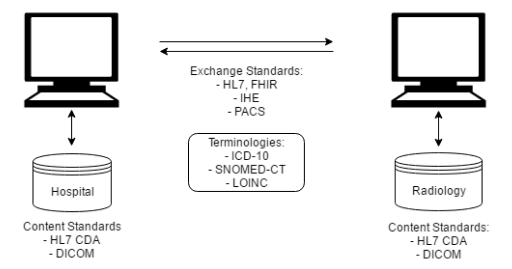
\includegraphics[width=0.80\textwidth]{img/content_exchage_standards.PNG}
	\caption{Use of content and exchange standards }
	\label{fig:content_exchage_standards}
\end{figure}

\paragraph{\textbf{Health Level 7 (HL7) -}}
As mentioned previously, the HL7 message (see table \ref{tab:hl7_2_4}) is also a format of exchange. The number seven on referees to the layer’s of the OSI model (Application, Presentation, Session, Transport, Network, Data Link and Physical) \citep{iso1994iec}.

These messages can be exchange by different protocol layers, but the most used are LLP (Lower Layer Protocol) also know as MLLP (Minimal Lower Layer Protocol) and HLLP (Hybrid Lower Layer protocol).  Both of them can be exchanged using a TCP/IP protocol. The LLP is the most used to transmit messages in a non-encrypted way on a local network (hospital cases). The HLLP has the advantage of incorporate error detection and verification by using “checksums” at the end of the messages, however is just used for non-trustful transportations \citep{grieve2012hl7}. Although the MLLP is the most used, the HTTP can be one alternative to add authorization (username/password).


\paragraph{\textbf{Fast Healthcare Interoperability Resources (FHIR) -}}
Is the last version of HL7 messages and combines all the features from the previous versions. It is easily implemented due to a set of components called resources. The resources can be based on administrative content, such as patient information, healthcare providers, medical or other type of devices used, locations or clinical content like medications, diagnostics, financial and others. However, there are more resources for workflow or clinical reasoning that can be represented on various formats like XML, JSON and Turtle (RDF) \citep{FHIR2017}. In the next image is presented an example of a patient (resource) FHIR file.

\begin{figure}[H]
	\centering
    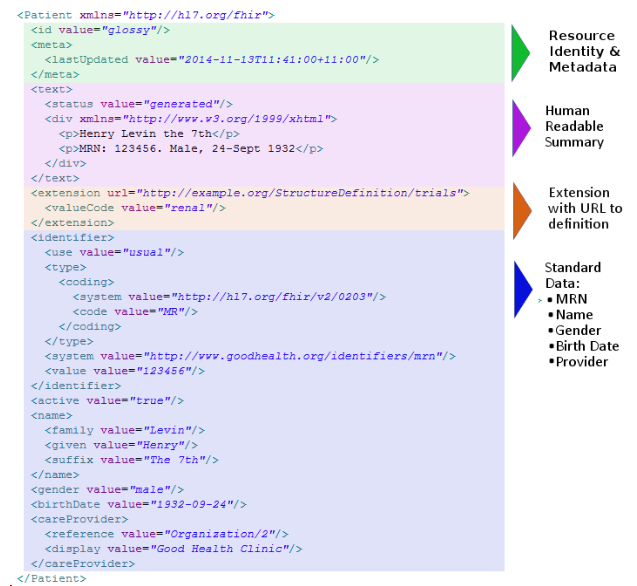
\includegraphics[width=0.9\textwidth]{img/fhir_patient.PNG}
	\caption{Example of a FHIR Resource: Patient \citep{FHIR2017}}
	\label{fig:fhir_patient}
\end{figure}

This message format can used on different platforms, from mobile phone applications to EHR data sharing, with a strong emphasis on web standards (JSON, XML, HTTP, etc) and with RESTful architecture support.
  
Also some examples of use cases for this standards are PHR, where the patient’s can check their data by using calls to the RESTful API (returning XML or JSON data) from a mobile or web portal application. It allows \ac{XDS} integrated with the IHE standards and decision support. For example, in the prescription of drugs, is possible to check drug interaction with other drugs, following safety guidelines - this type of decision support come from an engine on the system interface that makes use of the FHIR messages. The resources are based on Pareto principle, also known as 80/20 rule, that states that 80\% of the effects come from 20\% of causes, in FHIR case, it will only include a element if 80\% of the systems will implement it \citep{hl7fhir2017}. An element is the base type for all the sets included on a resource, and are represented by an ID code and an extension (additional content defined by implementations).   

\paragraph{\textbf{Integrating the Healthcare Enterprise (IHE) -}}
IHE is a non-profit organization established in 1998 by a consortium of radiologists and IT experts \citep{IHE2018}. It is a set of guidelines with specifications, called “Integration Profiles/Technical Frameworks” that define how the workflow should be inside of the hospital to improve the integration, interoperability and performance/efficiency of healthcare systems - how the systems share information inside of an organization. This framework is expanded every year with new updates and information. Furthermore, it promotes the use of standards like DICOM or HL7. Has a group of domains for each medical area that requires the use of an information system, like radiology, pathology and laboratory, cardiology, the IT infrastructure of the organization and many more. Inside of each domain there are different profiles. 

\begin{figure}[H]
	\centering
    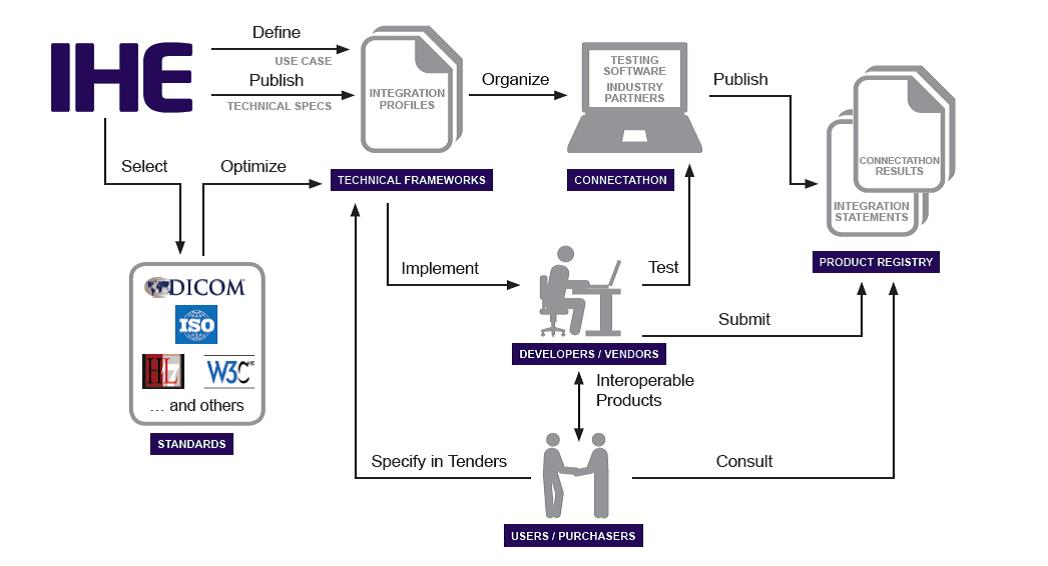
\includegraphics[width=1\textwidth]{img/IHE_process_flowchart.jpg}
	\caption{IHE methodology process flowchart}
	\label{fig:IHE_process_flowchart}
\end{figure}


\paragraph{\textbf{Digital Imaging and Communications in Medicine (DICOM) and Picture Archiving Communication System (PACS) -}}
DICOM is a standard for storing, retrieve, print, processing, transmitting and display digital images and respective information between imaging medical devices and workstations. It has protocols for the different image modalities like Computed Tomography (CT), Magnetic Resonance (MR), radiography, ultrasonography, among others.\\

The DICOM file is divided in two parts, the header with metadata information and the image data. Is based on a Service-Object Pair (SOP) Class, that defines a certain functionality consisting of a combination of a Service and an Object, which make up a pair - that pair can be Image Storage as a service and the MR or CT image as a object \citep{DICOM2018}. The images data are usually compressed with a lossless compression algorithm like GIF and PNG formats and also using lossy compression, for example JPEG2000, JPEG, TIFF formats - depending on what will be outcome usage of that file - medical supervision, presentation on websites or \textit{Microsoft PowerPoint}, teaching files, publications and many others \citep{varma2013}. This need of compressing images is due to the huge amount of data that the different modalities can produce, for example, one DICOM file (.dcm) can have 5 GB of size

\begin{figure}[H]
	\centering
    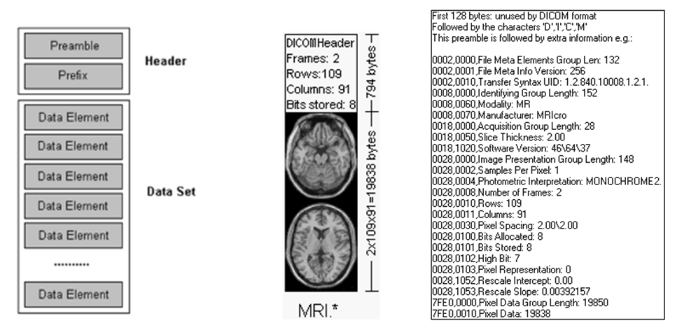
\includegraphics[width=1\textwidth]{img/data_dicom_file.PNG}
	\caption{Data content from a DICOM file}
	\label{fig:data_dicom_file}
\end{figure}


This files are saved in a system called \textbf{PACS (Picture Archiving Communication System)}. This system can provide storage and access to the images scanned from the different modalities and it is composed by the acquisition devices, communication network, archive system and visualization stations.

\subsubsection{Terminologies, classifications and nomenclatures: ICD, SNOMED, LOINC, MeSH, UMLS }
The basis of a clinical information system is the encoding of the medical terms. Having a controlled terminology avoid the developers from re-inventing the wheel and allows the systems to easily communicate with each other since these codes can be understood by the different systems, but unfortunately nowadays one of the most important basis of a EHR still being ignored and the developers continue using their own codification. This can happen due to non-adaptation or no knowledge of these standards to implement on the system that is being created. Some of the most specific and most used clinical terminologies are ICD, SNOMED, LOINC, but each one of them were created to meet and solve specific requirements. These terminologies are often divided in classification groups like type of disease, body system or anatomy and present a hierarchical order. Also, they are used to facilitate the input of medical data, like the SNOMED or LOINC standards and other standards are used to classificate and retrieve data from a system, like ICD. Normally these terminologies are connected to each-other. \citep{Bowman2005CoordinationOS}

\paragraph{\textbf{International Classification of Diseases (ICD) -}}
ICD is the international standard for identification of diseases, disorders, injuries and other related health conditions (classification system), that can be used for storage, retrieval, sharing and analysis of health information between hospitals, countries and also making data comparison of diseases during different periods of time. It is mostly indicated for clinical and management use and offers a coding information for the different diseases to be used into the systems. ICD facilitates information retrieval for secondary data purposes.

\begin{figure}[H]
	\centering
    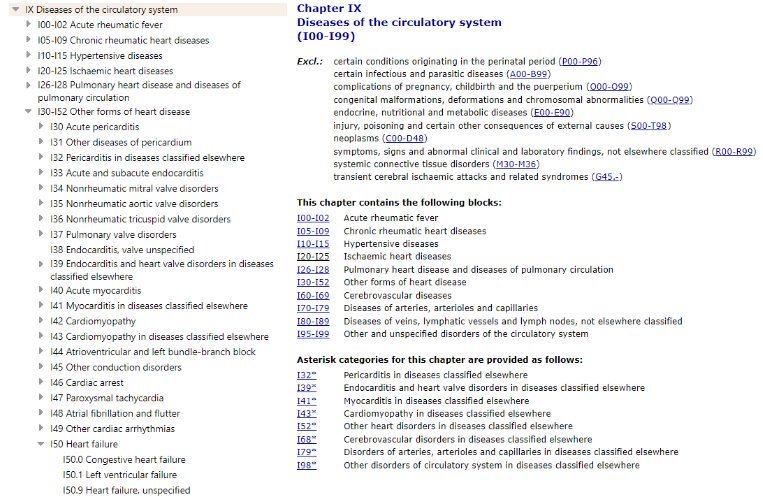
\includegraphics[width=1.1\textwidth]{img/icd.PNG}
	\caption{Examples of ICD-10 codes for circulatory systems.}
	\label{fig:icd_10}
\end{figure}

The actual version of ICD is in the tenth version, endorsed in 1990. Currently it has 16,000 codes to be used. Will be updated to version 11 in 2018. \citep{ICD2018}


\paragraph{\textbf{International Classification of Diseases - Clinical Modification (ICD-CM) -}}
Some nations expanded the code from ICD to have more information about clinical terms, adapting the nomenclature to their own systems. The versions are dependent from each country, and some editions can reach the  86,000 codes, comparing with the 16,000 from the international version. \citep{ICDCM2018}


\paragraph{\textbf{Systematized nomenclature of Medicine - Clinical Terms (SNOMED-CT) -}}
The SNOMED-CT is a comprehensive coding system (terminology system) and was created to describe and define patient data diagnosis when inserting information on a EHR. It allow the healthcare professional to use natural medical vocabulary and checking relationships inside of the desired medical term, like findings’ positions. \citep{SCT2018} It was released in 2002 and has more than 100,000 codes, concepts and other abbreviations. 

All these terms and respective codes can be found at SNOMED-CT terminology server: \url{https://snomed.terminology.tools}.

\begin{figure}[H]
	\centering
    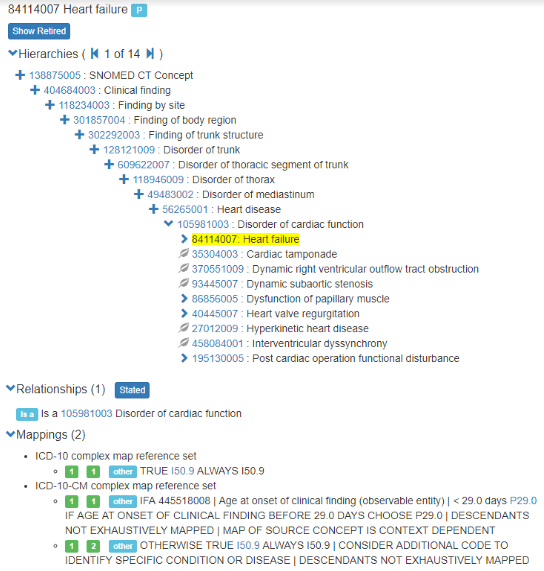
\includegraphics[width=0.95\textwidth]{img/snomed.PNG}
	\caption{Examples of diseases of circulatory systems codes in SNOMED-CT terminology server.}
	\label{fig:snomed_ct}
\end{figure}

\paragraph{\textbf{Logical Observation Identifiers Names and Codes (LOINC) -}}
LOINC is a naming system for tests and observations, that define codes for clinical measurements like vital signs, ECG, PHQ-9 questionnaire and many others or codes for laboratory tests results, such as hematology, toxicology, cell counts. In a easy interpretation if there is “anything that is possible to test, measure or observe about a patient” \citep{Loinc2018}, it will be present on LOINC. Technically, it makes use of the HL7 context message to retrieve information and is currently maintained by the Regenstrief Institute.\\

An example of LOINC code 806-0: \citep{LoincTERMS2018}
\begin{itemize}[noitemsep]
\item \textbf{Fully-Specified Name (FSN):} Component Analyte: Leukocytes: NCnc(Number concentration): Pt(Point in time): CSF(Cerebral Spinal Fluid): Qn(Quantity): Manual count
\item \textbf{Long Common Name (LCN):} Leukocytes [\#/volume] in Cerebral spinal fluid by Manual count
\item \textbf{Short Name:} WBC \# CSF Manual
\end{itemize}

\paragraph{\textbf{Medical Subjects Headings (MeSH) -}}
The MeSH terms are a special kind of terminology where all the medical literature relative to that term are indexed. It structures the medical terms hierarchically and permits searching those in a different levels of specificity. It is not used as a patient coding system, but it has a central role in the UMLS \citep{hammond2014standards}, explained below. It was created in 2005 and is maintained by the US National Library of Medicine.

\begin{table}[H]
	\centering
\caption{Hierarchical structure for "Medical Informatics" MeSH term}
\label{tab:mesh}
\begin{tabular}{l}
\toprule[2pt]
\begin{lstlisting}[language=octave]
Information Science [L01]
	Informatics [L01.313]
		Computational Biology [L01.313.124]
        	Consumer Health Informatics [L01.313.187]
        	Dental Informatics [L01.313.249]
		Medical Informatics [L01.313.500]
            			Health Information Exchange [L01.313.500.500]
            			Medical Informatics Applications [L01.313.500.750] 
            			Medical Informatics Computing [L01.313.500.875] 
		Nursing Informatics [L01.313.650]
		Public Health Informatics [L01.313.750]

\end{lstlisting}
\tabularnewline \bottomrule[2pt]
\end{tabular}
\end{table}


\paragraph{\textbf{Unified Medical Language System (UMLS) -}}
UMLS is a research and development program initiated in 1992 by the US National Library of Medicine and can be defined as the compendium of all the terminologies mentioned before, ontologies, files and software. Is a system that search the different terminologies repositories and enable the development of applications that can understand medical languages, by mapping the different vocabularies and standards from one computer to another. This can help health professionals to retrieve and integrate biomedical information, since it can communicate with various systems and overcome the problems created by the differences of terminologies usage in the different applications.It makes use of tree different knowledge sources, Metathesaurus, Semantic Network and the Specialist Lexicon.


\subsubsection{Information Modelling: HL7 RIM and openEHR }
One of the most important standards currently on healthcare IT area is the information modelling. It describes how the information should be structured. In healthcare, lot of applications were developed and the underlying information model for saving clinical information was left to be developed solely by system implementers. This guides to a challenge on how to connect the different information from different systems or even various devices in one database. \citep{huff1995event} All this variety of data input leads to a big problem - not having a functional and consistent information model dealing with all the different situations. To solve this problem, some standards emerged, like openEHR and HL7 RM. \citep{piho2015business}

\paragraph{\textbf{HL7 Reference Information Model (RIM) -}}
The HL7 organization has developed a reference information model to specify the entities, roles, participations, acts and the data elements associated, to make the different healthcare systems sustainable to communicate and exchange data with each other. For example, it represents all the physical objects like hospitals or devices and persons as entities, and events like observations or procedures as acts. It makes use of other standards from HL7, like the v2 or v3 messages and the CDA, and identifies the life cycles of all events that those messages can carry.

\paragraph{\textbf{OpenEHR -}}
Has a similar approach of HL7 RIM, using a multi-level modeling methodology. These models are constituted by the base information structure for the EHR systems. OpenEHR is divided in two-levels: the first level is composed by the reference model, that gives the software specifications, such as the generic data types – text, quantities, booleans - and data structures – list, tables, trees \citep{sinha2012electronic}\citep{cresswell2013ten}. In the second level are presented the archetypes and templates. The archetypes have a Lego\texttrademark{ } model approach, giving elementary concept base to create structures - the templates. Also, the archetypes can be shared and re-used, so it is not necessary to create new archetypes for different templates. Some of the \textit{pros} of using openEHR in EHR systems are the possibility of separating the information model from the content model.\\

The main difference between both information models reside in the fact that openEHR has the separation of semantics domain, that allows to involve more the healthcare professionals and IT developers in the implementation of the system, having much more solid reference model when comparing with HL7, which is more abstract. This causes a not so easy involvement in the HL7 approach by the previous community, since is more directed to application developers. Either these RMs differ on the constraints used - openEHR makes use of templates and archetypes, that gives freedom to a community to work together in the implementation of new archetypes, and on the HL7 side, this is made with different types of profiles (artifacts) as Domain Message Information Model (DMIM), Refined Information Model (RMIM) and Common Message Element Types (CMET) \citep{Grieve2016vid} that requires a more directed IT background and the creation of new profiles are not so open as in openEHR. It makes use of a big part of the information already contained in the HL7 and FHIR specifications. \\



\begin{table}[h]
\centering
	\caption{Comparison of reference models and artifacts between different technologies \citep{Grieve2016vid}}
	\label{tab:RM_comparision}
	\begin{tabular}{lll}
		\toprule[2pt]
		\cmidrule(r){1-2}
		\textbf{Technology}    & \textbf{Reference Model} & \textbf{Constraints} \\
		\midrule[2pt]
		HL7 v3  & RIM & DMIM, RMIM, CMET \\
		\midrule
		FHIR & Resources & Profiles \\
		\midrule
		OpenEHR & RM & Archetypes and Templates \\
		\bottomrule[2pt]
\end{tabular}
\end{table}



\section{Application Programming Interface (API)}
An API sets the path and protocols of two or more different computers that can communicate in a common language and in understandable way to each other, in order to build software applications. The basis of this communication is called a web service, which is identified by a \ac{URI}. An API is composed by a set of programming functions that can be accessed over HTTP methods, mostly for request and response calls. These calls are usually under \ac{JSON} or \ac{XML} formats and can be made by \ac{SOAP} or \ac{REST} models. 
This kind of functionally is created when a software company has the intention of having external developers or teams to develop products by themselves, but still associated at their service.\\

The most commonly used HTTP methods are:
\begin{itemize}[noitemsep]
\item \textbf{GET} - Read only access to some resource.
\item \textbf{POST} - Update or create a new resource.
\item \textbf{PUT} - Create a new resource.
\item \textbf{PATCH} - Update a new resource.
\item \textbf{DELETE} - Remove a resource.
\end{itemize}

Every time there is a request from one machine to another machine, this is followed by a internal HTTP response. Each request and response have respective identifying codes, that can vary from 100 to 500 and are codified in ASCII format. When a request is made, a similar message to figure \ref{fig:http_methods} is retrieved.

\begin{figure}[H]
	\centering
    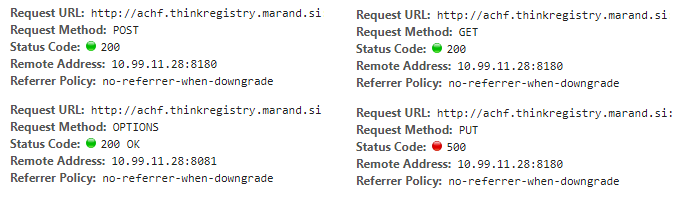
\includegraphics[width=1\textwidth]{img/http_methods.PNG}
	\caption{HTTP methods}
	\label{fig:http_methods}
\end{figure}

The values of the responses (status code) have different meanings. A successful request would get the code 200 ("200 OK", "201 Created"), a redirection would get the code 300( "301 Moved Permanently", "303 See Other", "304 Not Modified") and a bad request would get the code 400 (the requested message could not be understood by the server- "404 Not found", "412 Precondition Failed") or the famous 500 error code ("500 Internal Server Error"). \citep{sundvall2013applying} Usually these status are codified as:

\begin{itemize}[noitemsep]
\item \textbf{1XX} - informational
\item \textbf{2XX} - success
\item \textbf{3XX} - redirection
\item \textbf{4XX} - client error
\item \textbf{5XX} - server error
\end{itemize}



\begin{figure}[H]
	\centering
    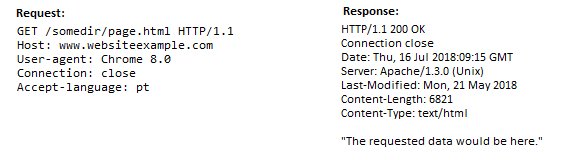
\includegraphics[width=0.9\textwidth]{img/http_request_reply.PNG}
	\caption{HTTP methods - request and response}
	\label{fig:http_request_reply}
\end{figure}

Lately, a huge number of organizations started to prefer REST architecture instead of SOAP protocol, due to the less bandwidth and payload required by REST during communications - sending a request in JSON format is less "heavier" than a request in XML format.

\subsection{REST API}
REST is a standard for web based architecture which uses the HTTP protocol and methods for communication between machines. The basis is simple: A request is sent to another machine - if the request was understood, it should retrieve a response. The most typical format on REST architectures is JSON.

\begin{figure}[H]
	\centering
    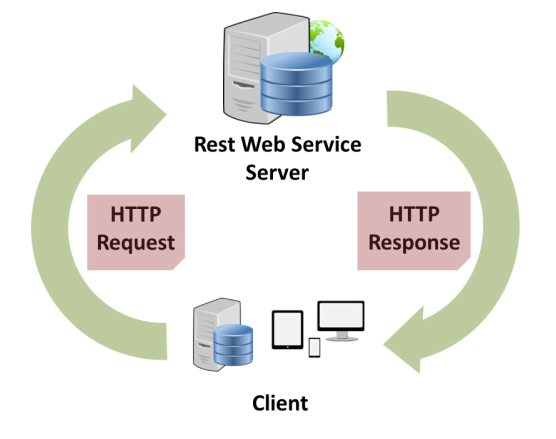
\includegraphics[width=0.5\textwidth]{img/rest_webservice.PNG}
	\caption{REST Web Service}
	\label{fig:rest_webservice}
\end{figure}

When mentioning a REST API, it means that it is a programming interface based on a RESTful web service (a web service based on a REST architecture). This will be the way of communication used in the implementation part of the script while exchanging data with the different web repositories. In a REST request, is provided an URI combined with one of the desired of HTTP methods. For example, in the figure \ref{fig:URI_methods} is possible to see how to get a file using REST API.  

\begin{figure}[H]
	\centering
    
\includegraphics[width=1.05\textwidth]{img/URI_methods.PNG}
	\caption{HTTP Method and URI}
	\label{fig:URI_methods}
\end{figure}

An example of an open REST API for electronic health records based on openEHR can be accessed at: \url{https://www.ehrscape.com/api-explorer.html} and an OpenEHR REST API from openEHR foundation can be found at: \url{https://www.openehr.org/releases/ITS/Release-0.9.0/docs/index}

\newpage 
\section{OpenEHR}
OpenEHR (ex-GEHR - Good European Health Record and later Good Electronic Health Record) is a specification and non-profit foundation that focuses on standards for managing clinical data. It was created in 2000 by a virtual community of doctors, health and information technology professionals from Europe, Brazil and Australia \citep{openEHRhist2002}, but the research and development process of understating how a EHR works, remotes from 1985 in a more focused attention to the European territory. The "motto" of this community is: “The transformation of health data from physical format to electronic format, thus ensuring universal interoperability between all forms of electronic data” \citep{openEHR2018}. OpenEHR is also a free open-source platform which provides rules of how to work, share and store health data with the principal idea of separating this data from applications as an agnostic approach \citep{kalra2005openehr}. Some of the benefits of using this platform are the possibility of working with medical information at the same semantic level, lowering the problems with mismatched clinical information models, strengthening the interoperability and making possible the use of analytic functions, such as research querying and decision support. The target is to create and design a way for an universal and shareable EHR \citep{Madsen2010}.  It is also possible to build an independent data repository for this EHR that does not need to know what kind of information will get in the beginning, because it can be modeled for what the healthcare institutions requires as 
the needs appear. OpenEHR has his own international repository, called Clinical Knowledge Manager (CKM), with all the approved archetypes and templates, which are updated when needed by medical and informatics experts, after a common approval. Also, to meet specific requirements some national CKMs were also created \citep{openEHRCKM}.

\begin{figure}[H]
	\centering
    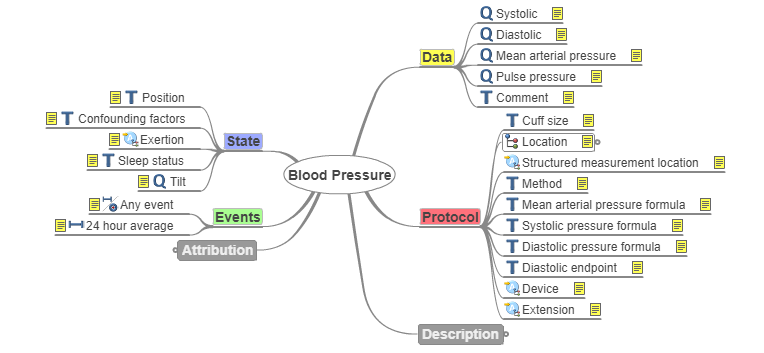
\includegraphics[width=1\textwidth]{img/bp_openehr.PNG}
	\caption{ Blood Pressure archetype - mindmap view (OpenEHR CKM)}
	\label{fig:bp_openehr}
\end{figure}


\subsection{Architecture}
The architecture of openEHR is complex, but covers the bigger part of how an EHR should behave. Is updated several times a year by medical and informatics experts. New documentation releases can be found at: \url{http://www.openehr.org/programs/specification/latestreleases} \\

Currently, is composed by two main levels. Each level contains different information models and specifications:
\begin{itemize}[noitemsep]
\item \textbf{Reference Model (RM)} - root and basis of the system.
\item \textbf{Archetype Model (AM)} - has the content for clinical or administrative data.
\end{itemize}
When relating the openEHR packages, besides the other mentioned models, the \textbf{Service Model (SM)} is also included and defines the basic services for integration with other health care information environments, like tools or APIs. 


\subsection{Two level modeling (RM and AM)}
The two level modeling approach on openEHR allows to separate the information model from the content. The first level is composed by the Reference Model (RM), and this is the only part implemented on software. The second level has all the information related with the clinical information, translated in archetypes - the Archetype Model (AM). In figure \ref{fig:openehr_components}, are represented the AM, RM and SM information models, and the respective available packages within the models. 

\begin{figure}[H]
	\centering
    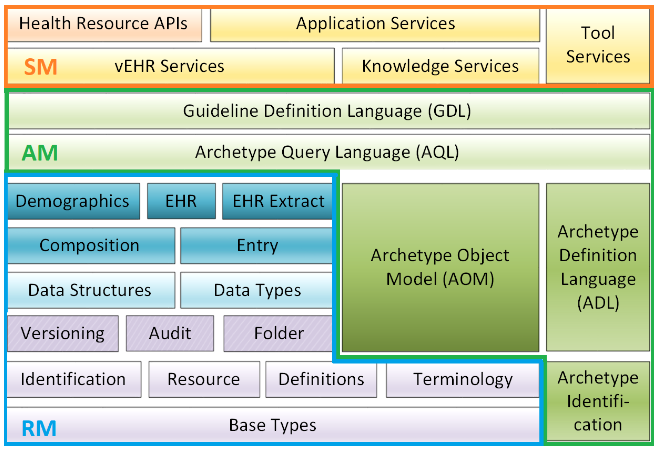
\includegraphics[width=0.8\textwidth]{img/openehr_components.PNG}
	\caption{openEHR package structure components}
	\label{fig:openehr_components}
\end{figure}

The service model (SM) provides all the access around the EHR system, like back-end services, request and reply services like \ac{SOAP} or \ac{REST} \ac{API}’s and other source files.
	
The Reference Model (RM) is the base model and have a Lego\texttrademark{ } analogy approach. It provides all the basic information to the upper levels, like various packages with knowledges resources, data types, versioning and many others. In this model is also presented the “EHR” information model (the core part of openEHR), which include the “\textit{ehr}” and “\textit{composition}” packages and define the content and context of main concepts like “EHR”, “COMPOSITION”, “SECTION” and “ENTRY”.

The “Folder” package have all the compositions based in some similar parameter or criteria. It can be the dates between some clinical specialities, some physician folder containing information about patients or even a clinical team folder. The "EHR" package is also responsible by the "EHR ID", "versioning", "contributions", "access control", "status" and has a "COMPOSITION" (C) which manages documents by date and hour and contain all the clinical and administrative information of the EHR. Each composition is inside of a "VERSIONED COMPOSITION" (VC) package (also called versioned\_object), that makes the version control of each composition (figure \ref{fig:openehr_structure}). The behavior is similar to a git repository, since it makes the storage of all the different compositions that have been saved and when requested, retrieves the versions that were saved too.


\begin{figure}[H]
	\centering
    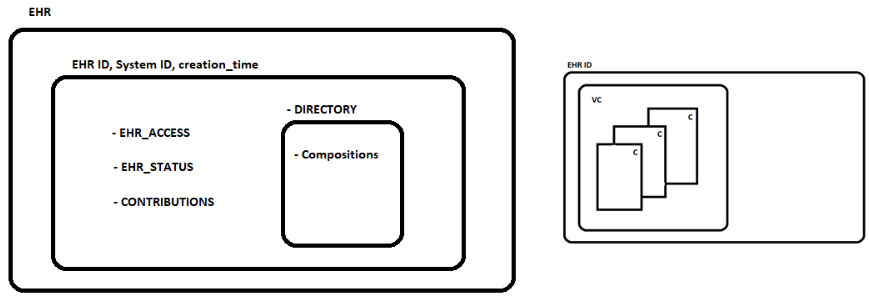
\includegraphics[width=1.1\textwidth]{img/openehr_structure.PNG}
	\caption{OpenEHR "EHR" structure}
	\label{fig:openehr_structure}
\end{figure}

Then, a “COMPOSITION” can have one or more “SECTIONs” that will make the organization and structure of all the EHR’s content with an “ENTRY”, that can be divided by “admin\_entry” and cares about all the information to set up the clinical process, but which is not clinically relevant, or “care\_entry” (“observation”, “evaluation”, “instruction” and “action”) that retrieves the clinical information about the patient.

The care entries are what define the kind of care delivered and are composed by \citep{openEHRCKM}:
\begin{itemize}[noitemsep]
\item \textbf{Observation:} Makes the record of a direct observation or measurement, such as body weight, blood pressure or having the record the historical retrospective from the patient.
\item \textbf{Evaluation:} Can be a clinical opinion like a goal or a diagnosis, that have been measured or gathered and show clinical evidence.
\item \textbf{Instruction:} It is used to record a clinical activity, providing a set of rules and instructions, and includes cancellation or postponement. It will have an action as a reply. Can be a medication order, a service request, laboratory test, etc.
\item \textbf{Action:} Record a step in carrying out a clinical activity, including cancellation or postponement. Can be a reply to an instruction. 
\end{itemize}

OpenEHR defined a decision algorithm for choosing the correct reference model when creating an archetype, and it can help on the governance of those artifacts. This algorithm is shown on the figure \ref{fig:decision_alg_arch} and can help to have a wider view of all the components inside of the EHR along with how to create and model an archetype.

\begin{figure}[H]
	\centering
    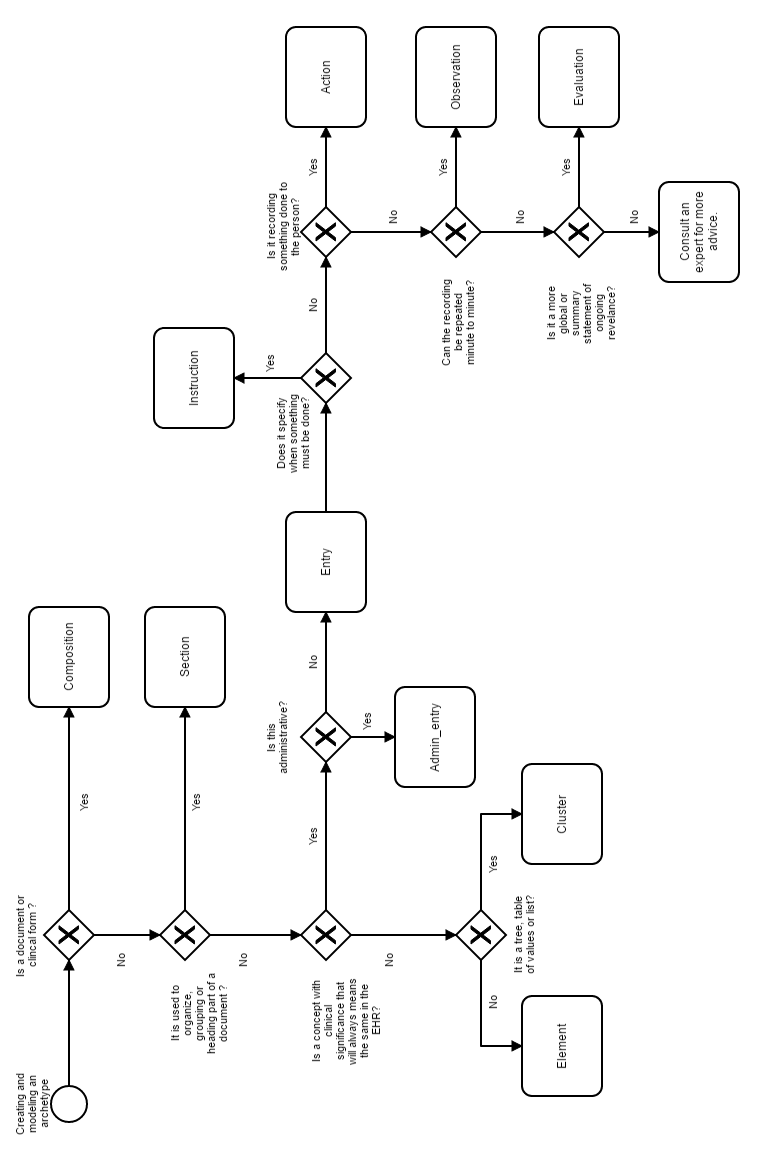
\includegraphics[width=1.05\textwidth]{img/decision_alg_arch.PNG}
	\caption{OpenEHR decision algorithm - adapted from openEHR reference model class (Heard, 2010) }
	\label{fig:decision_alg_arch}
\end{figure}

Every entry mentioned above, has a data type. The main types are:
\begin{itemize}[noitemsep]
\item \textbf{Text} - (dv\_text, dv\_coded\_text);
\item \textbf{Quantity} - (dv\_ordinal, dv\_count, dv\_quantity); 
\item \textbf{Date\/time} - (dv\_date\_time, dv\_duration); 
\item \textbf{Multimedia} - (dv\_multimedia); 
\item \textbf{Boolean} - (dv\_boolean, dv\_state); 
\item \textbf{Uniform Resource Identifier (URI)} - (dv\_uri).
\end{itemize}

In the figure \ref{fig:openehr_comp_struct} is possible to see how the different data types are being used in each item of the entries (e.g. blood pressure and medication management). 

\begin{figure}[H]
	\centering
    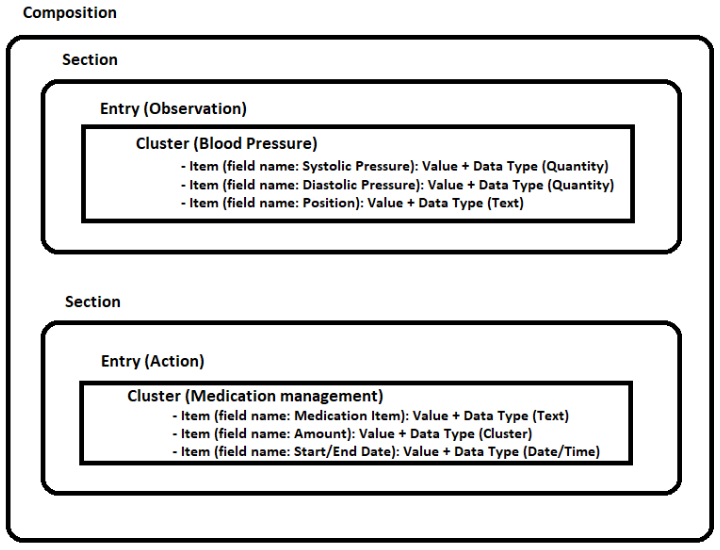
\includegraphics[width=1\textwidth]{img/openehr_comp_struct.PNG}
	\caption{OpenEHR composition structure}
	\label{fig:openehr_comp_struct}
\end{figure}

Each entry has a cluster, a complex entry of data such as a test result for blood pressure. Inside of the cluster there are different items. They represent the single input for each field, for example the cluster “blood pressure” will have the “systolic” and “diastolic” inputs. An item always have a field name, value and data type. Also, a “composition” can have different “contributions” made on different dates or times. It can be an event (patient contact), acquisition (test results) or correction of an event (correction of the previous patient contacts).

The archetype model (AM) contains all the modules and packages, such as archetype definition language (ADL), archetype and template, which describe the artifacts used within openEHR. It provides all the rules regarding how to build these artifacts. 

All these information systems based on openEHR are being implemented using UML notation with class specification. The main idea is to provide the same way of understanding and communication for the groups involved on the development. 

\subsection{CKM}
When creating a clinical information system is necessary to have a clinical knowledge repository to save all the information regarding the data modeling on use. The best way to be sure that all the systems based on openEHR are getting the same information using archetypes is by a Clinical Knowledge Manager (CKM). CKM is an online repository of clinical content (archetypes and templates) and also a collaboration tool, where is possible to adapt specifications to the different artifacts. The openEHR foundation has an international repository of archetypes and templates that is being maintained and updated when necessary by an online group of health care and informatics professionals. The CKM will be explained with more details in the chapter 3 (Study I - OpenEHR CKM).

\subsection{Clinical Models}
For several years, a lot of applications have been made to deal with clinical data that should address innumerable purposes. This models should be capable of formalizing, structuring and standardizing data elements for clinical use, having in attention the structures and relationships of this usage. The clinical models are responsible to make the organization of health information by combining the knowledge of health care professionals, specification of data elements and relationship between them, and terminology to be used in information models that will be deployed on different formats, such as HL7 or openEHR. In case of openEHR, it offers archetypes and templates and those are connected to terminology (f.e. templates have terminology connected to ICD10, SNOMED-CT, LOINC and many others). One of the biggest and common problems with clinical models is the mismatched information for the same action between different platforms, like a desktop application or a mobile application for both patient and healthcare professional. An example can be the different way that a medication name and respective prescription can be saved or retrieved from these platforms.

\begin{figure}[H]
	\centering
    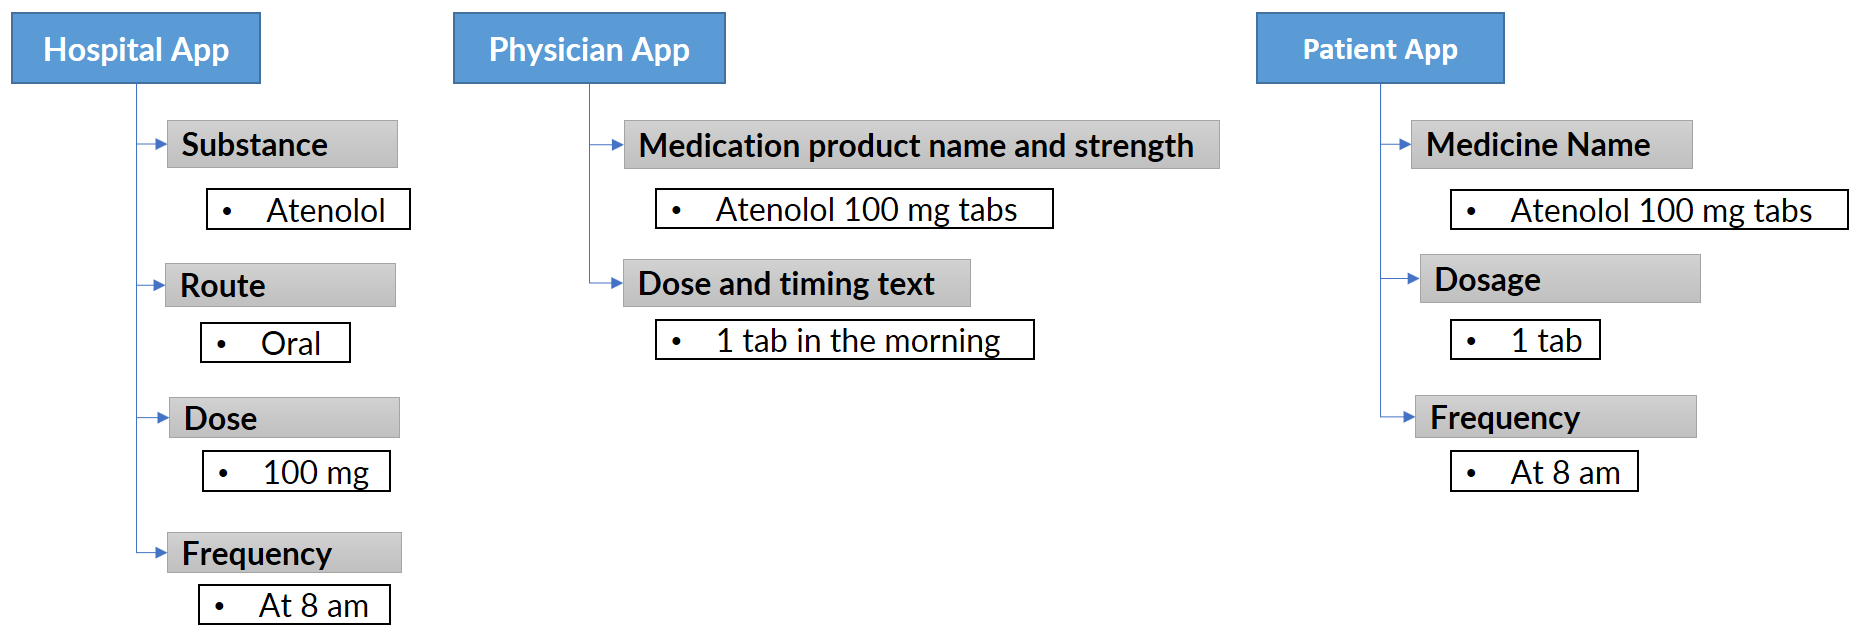
\includegraphics[width=0.95\textwidth]{img/mismatched_IM.PNG}
	\caption{Mismatched information models between different applications (adapted from Ian McNicoll presentation on openEHR Day London 2017)}
	\label{fig:mismatched_IM}
\end{figure}

In the case of using openEHR resources, this dilemma is easily solved, due to all the information will be saved or retrieved exactly the same way on each application.

\subsection{Archetypes, Templates, ADL and AQL}
The artifacts/resources of openEHR are the archetypes and templates. They are directly connected, and in a simple way, is possible to consider that one template is a set of archetypes, but the template is by himself, a giant and specialized archetype. The Archetype Definition Language (ADL) is defined by the openEHR foundation as \textit{“ an abstract human-readable and computer-processable syntax and can be hand-edited using a normal text editor”}. It is the language used inside of the archetypes. Since 2002, ADL has changed from version 1.2 to version 2.0.\\

\begin{figure}[H]
	\centering
    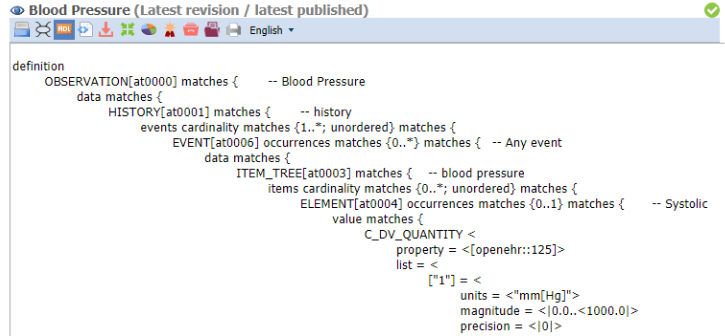
\includegraphics[width=0.95\textwidth]{img/bp_adl.PNG}
	\caption{ADL for “Blood Pressure” archetype (from openEHR CKM)}
	\label{fig:bp_adl}
\end{figure}

The Archetype Query Language (AQL) is what makes possible querying the ADL. The possibility of querying archetypes with the AQL offers many benefits, because it is prepared to query a database that is perfectly defined by the openEHR RM model, against querying one proprietary database with \ac{SQL} that is being filled with information from a specific form, with a huge possibility of various elements. In the next figure is possible to see what an AQL query looks like: \\

\begin{table}[H]
	\centering
\caption{Querying diastolic and systolic input values between 160 and 180 mmHg from blood pressure measurement archetype}
\label{tab:bp_aql}
\begin{tabular}{l}
\toprule[2pt]
\begin{lstlisting}[language=SQL]
select
    e/ehr_id as EHR_ID,
    a_a/data[at0001]/events[at0006]/data[at0003]/items[at0004]/value as Systolic,
    a_a/data[at0001]/events[at0006]/data[at0003]/items[at0005]/value as Diastolic
from EHR e
contains COMPOSITION a
contains OBSERVATION a_a[openEHR-EHR-OBSERVATION.blood_pressure.v1]
where
    a_a/data[at0001]/events[at0006]/data[at0003]/items[at0004]/value/magnitude>=180 or
    a_a/data[at0001]/events[at0006]/data[at0003]/items[at0005]/value/magnitude>=160
\end{lstlisting}
\tabularnewline \bottomrule[2pt]
\end{tabular}
\end{table}

\newpage
\subsubsection{Understanding the archetypes}
To understand the way the archetypes are based and how they work, is necessary to consider the basics of ontology, which are defined as “a set of concepts and categories in a subject area or domain that shows their properties and the relations between them” (Oxford 2018). Thus, an archetype is the key feature of separation between information models and domain models, that defines how to capture clinical data \citep{Beale2007}. It is a set of data elements and other data groups with formal definition of knowledge domain, for an healthcare information system and can be reusable in different situations.

An archetype can be considered as the basis of a form and provide a standard clinical content specification \citep{Madsen2010}. For example, the archetype “Blood Pressure” include all the data slots that can be used on blood pressure observation form. Some of these points can be repeated on others archetypes that are under the same topic. Is also possible to compose or decompose an archetype and include the data slots from it in another archetype, like the case of “Fetal Heart Rate” archetype being decomposed and including some of these elements into the “Heart Rate” archetype, specializing it in this way. If necessary, is possible to add external terminologies to them, such as IDC-10, SNOMED, LOINC, among others.

There are four types of archetypes, some of them mentioned previously: 
\begin{itemize}[noitemsep]
\item \textbf{“Composition”} that contains all the information stored in a EHR and has “sections” with different \textit{archetyped} “entries” ; 
\item \textbf{“Section”}, correspondent to headings;
\item \textbf{“Entry”,} the unit of information, like systolic blood pressure, heart rate, etc. These entries are divided in four sub-types:
\begin{itemize}[noitemsep]
\item \textbf{Observations}; 
\item \textbf{Evaluations}; 
\item \textbf{Instructions}; 
\item \textbf{Actions};
\end{itemize}
\item \textbf{“Cluster”}, which contains archetypes for use into any “entry” or even another “cluster”.
\end{itemize}

Another relevant aspect of the archetype is that they are not a part of software or database of a system. They provide validation of data and the possibility of querying data by using AQL language, very similar to SQL. Although the openEHR CKM has a big repository of archetypes, in very specific cases, some of them needs to be rebuild to fill up the client requirements. Still, they are based and checked by clinical experts.

\subsubsection{Archetype specialization}  \label{sssec:AS}
When an archetype is called "specialized", it means that is based on a parent archetype, but it has a different format due to fulfillment of special requirements, which the parent archetype could not met. An example of it can be seen in the table \ref{tab:nyha_adl}, where the "nyha\_heart\_failure" archetype that has been specialized to "nyha\_heart\_failure-slo" to meet some special slovenian specification for the requirements of a client. An archetype of this type has present on the ADL format the announcement of being a specialization. 

\begin{table}[H]
	\centering
\caption{Intro of NYHA heart failure archetype - slovenian variant (ADL format)}
\label{tab:nyha_adl}
\begin{tabular}{l}
\toprule[2pt]
\begin{lstlisting}[language=XML]
archetype  (adl_version=1.4; uid=69453c5f-b816-40d9-98a4-a2a1a1164877)
           openEHR-EHR-CLUSTER.nyha_heart_failure-slo.v1

specialize
           openEHR-EHR-CLUSTER.nyha_heart_failure.v1

concept
           [at0000.1]
          
language
           original_language = <[ISO_639-1::en]>
\end{lstlisting}
\tabularnewline \bottomrule[2pt]
\end{tabular}
\end{table}

Since it is a specialization, these type of archetypes will be created in a more internal way and are not so shareable like the archetypes present at the international CKM, only if submitted to it and waiting for approval. Although there are some examples on the international CKM, the status of each one of these archetypes are draft of pre-draft.


\subsubsection{Understanding the templates}
One template aggregates and defines the data sets within the archetypes. When creating a template, this does not need the same amount of preparation and design used to create an archetype. it is dependent on the use case, speciality, domain and location, and make the definitions for the content of a form or report. In the figure \ref{fig:bp_arch_struct} is possible to see the structure of the “Measurement Blood Pressure” template.

\begin{figure}[H]
	\centering
    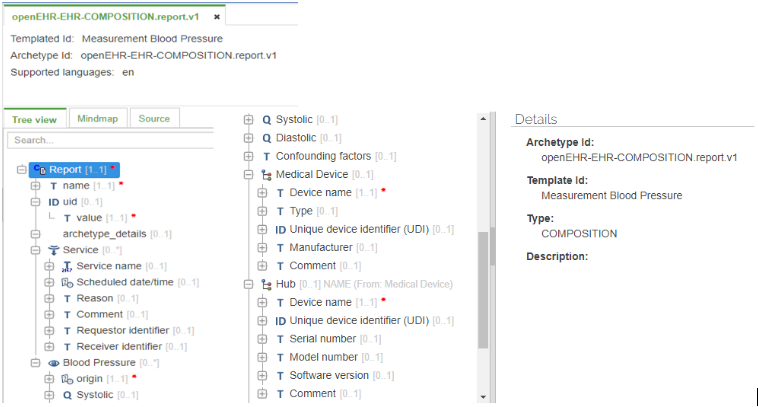
\includegraphics[width=1\textwidth]{img/bp_arch_struct.PNG}
	\caption{Structure of “Measurement Blood Pressure” template on EHRExplorer (Marand d.o.o) }
	\label{fig:bp_arch_struct}
\end{figure}

It is always necessary to have a root archetype (composition), which in this case is a “report” type. Then this composition needs to be fulfilled with specific archetypes for the use case of this template, that will fill up the slot-fillers, such as “Blood Pressure” (observation), “Service” (action),  Medical devices (cluster) and Hub (cluster). Is not necessary to have all the archetype data items if they will not be used. For that, is possible to constrain the options by changing the multiplicity of the occurrences (e.g. [0..0], [0..*], etc) making the mandatory items being optional or vice-versa. \citep{Beale2007}

There are two types of templates: \ac{OPT} and \ac{OET}. The pre-ADL2 version template (OET), is currently less used and only editable on Template Designer (Ocean Informatics). It only has the identification of the archetypes used to create the template. 

The other type is the operational template (OPT), which is a finished and compiled template that produces a flattened form expressed in XML, that will be read and used by a machine. It makes the joint point between semantic specifications and the different software files that can be used by developers, like XML Schema Definition (XSD), Java and C\# API’s, GUI screen forms and others.


\begin{table}[H]
	\centering
\caption{“Blood Pressure” archetype in “Measurement Blood Pressure” OPT template (XML format excerpt)}
\label{tab:bp_opt}
\begin{tabular}{l}
\toprule[2pt]
\begin{lstlisting}[language=XML]
  <archetype_id>
     <value>openEHR-EHR-OBSERVATION.blood_pressure.v1</value>
  </archetype_id>
  
              <term_definitions code="at0000">
                 <items id="text">Blood Pressure
                 </items>
                 <items id="description">The local measurement of arterial blood pressure.
                 </items>
              </term_definitions>
              
              <term_definitions code="at0001">
                 <items id="text">history
                 </items>
                 <items id="description">History Structural node.
                 </items>
              </term_definitions>
              
              <term_definitions code="at0004">
                 <items id="text">Systolic
                 </items>
                 <items id="description">Peak systemic arterial blood pressure  - 
                 	measured in systolic or contraction phase of the heart cycle.
                 </items>
              </term_definitions>
              
              <term_definitions code="at0005">
                 <items id="text">Diastolic
                 </items>
                 <items id="description">Minimum systemic arterial blood pressure - 
                 	measured in the diastolic or relaxation phase of the heart cycle.
                 </items>
              </term_definitions>
              
              
\end{lstlisting}
\tabularnewline \bottomrule[2pt]
\end{tabular}
\end{table}

The OPT is a dynamically created object from an OET template, which is based on openEHR archetypes. The workflow of archetype creation, until getting an OET and OPT templates is shown on figure \ref{fig:OET_OPT}, using one of the openEHR tools, ADL Designer, as a modeling and integration tool and Think!EHR platform, an "high-performance solution designed to store, manage, query, retrieve and exchange structured electronic health record data based on the latest release of openEHR specifications." \citep{t!ehr}.

\begin{figure}[H]
	\centering
    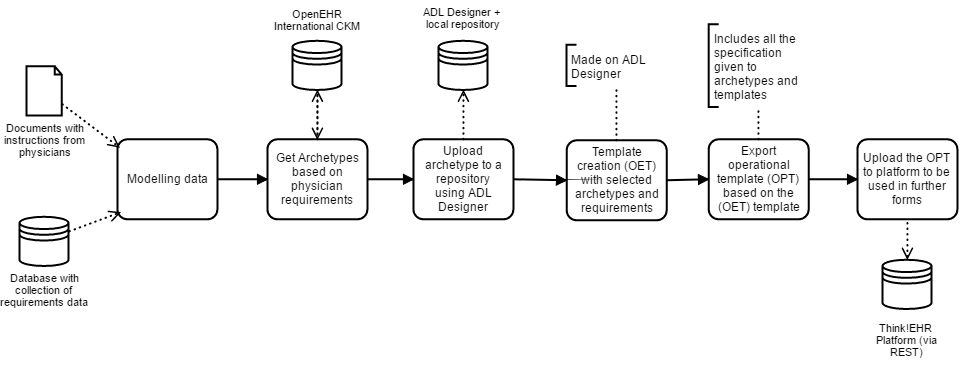
\includegraphics[width=1.1\textwidth]{img/OET_OPT.PNG}
	\caption{Archetype to template workflow using ADL Designer}
	\label{fig:OET_OPT}
\end{figure}



\subsection{Tools}
Since the international CKM is managed by an online community that can create, edit and publish artifacts, there are some modeling tools to help with the creation of archetypes and templates.\\ 

The current supported application is ADL Designer, an online tool created by Marand that allows to parse, serialize, flattening and validate the archetypes, and it is the tool that will be used in development part of this dissertation. Is compatible with the version 1.4 ADL archetypes and 1.4 OPTs. Also, it allows direct connection with other online repositories, like Github, Bitbucket, Google Drive, Dropbox, One Drive or local and central repositories like GIT or Subversion.\\ 

There are other desktop tools created by different companies (see table \ref{tab:tools} in the next page), such as Ocean Informatics’ Archetype Editor (AE) and Template Designer. Those were the most used tools and have been used since the beginnings of archetype modeling, but currently are not supported anymore. The archetype workbench is also a very useful tool that test the accuracy of the archetypes and their based relationship. All the existing tools can be downloaded from the openEHR modeling tools page. 
\vfill
~

\begin{table}[H]
\centering
\caption{ List of active openEHR related software and modeling tools (march 2018)}
\label{tab:tools}
\begin{tabular}{p{3.5cm} p{5cm} p{2cm} p{4cm}}
\toprule[2pt]
\textbf{Software name}                     & \textbf{Description}                                                                                                                                                                                                                                                                                                                    & \textbf{Technology}        & \textbf{Link for download}                                                                                \\ \midrule[2pt]
\textbf{ADL Designer}                      & The tool allows visual authoring of ADL 2 archetypes and templates including full archetype parsing, validation, flattening and serialization. Backward compatibility for existing ADL 1.4 archetypes and export to Operational Template (1.4 OPT) is also supported. Work with: ADL 2 archetypes, templates, ADL 2 OPTs, ADL 1.4 OPTs. & web (JavaScript, HTML etc) & \url{http://ehrscape.marand.si/designer/}                                                                      \\ \midrule
\textbf{Archetype Editor (AE)}             & The Archetype Editor is currently the main tool in use for authoring archetypes as found on openEHR CKM and elsewhere. It is Unicode-enabled and works with archetypes in any language. Work with: ADL 1.4 archetypes.                                                                                                                  & Microsoft VB.NET           & \url{https://www.openehr.org/download\_files/archetype\_editor/archetype\_editor\_2.8.972.1-windows\_32bit.exe} \\ \midrule
\textbf{Template Designer}                 & The Template Designer is the tool required for editing '.oet' (pre-ADL2) templates. .oet templates; ADL 1.4 OPTs; ADL 1.4 archetypes.                                                                                                                                                                                                   & Windows, .Net.             & \url{https://www.openehr.org/download\_files/TemplateDesigner/TemplateDesignerSetup\_2.8.94.2.exe}              \\ \midrule
\textbf{ADL2 workbench (AWB)}              & Reference model-driven visual IDE for parsing, compiling, analyzing, converting and editing archetypes and templates. Built on the reference ADL parser. ADL 1.4 (read), ADL 2 archetypes and templates (read/write).                                                                                                                   & Windows, Linux and Mac OSX & \url{https://www.openehr.org/downloads/ADLworkbench}                                                            \\ \midrule
\textbf{ADL2 command-line compiler (ADLC)} & A command-line version of the compiler used inside the ADL Workbench (AWB). ADL 1.4 (read), ADL 2 archetypes and templates (read/write).                                                                                                                                                                                                & Windows, Linux and Mac OSX & \url{https://www.openehr.org/downloads/ADLworkbench}                                                            \\ \midrule
\textbf{LinkEHR Editor}                    & The LinkEHR Editor works with multiple reference models and languages. Reference models can be plugged in in XML-schema or openEHR BMM (basic meta-model) format. .oet templates; ADL 1.4 OPTs; ADL 1.4 archetypes.                                                                                                                     & Java                       & \url{http://veratechnas1.synology.me:6969/linkehr/getlinkehr.html}                                              \\ \midrule
\textbf{ADL Text Editor Modes}             & ADL syntax plug-ins, syntax files and other support for text editors, including gvim/vim, emacs, Notepad++, Textpad, and Kate/KDevelop.                                                                                                                                                                                                 & Windows, Linux and Mac OSX & \url{https://openehr.atlassian.net/wiki/spaces/dev/pages/6553628/ADL+Text+Editors}                              \\ \bottomrule[2pt]
\end{tabular}
\end{table}


\section{Life cycles of projects}

Working on a project requires to pass every phase associated to it from the start until the finish phase line. All these phases compose the life cycle of a project. It is necessary to evaluate all the phases of the project, to know if it will be feasible to maintain and how to deal with them. Since the aim of this dissertation is related with software development, it will be presented a special framework that is commonly used on this area, the \ac{SDLC} \citep{wilcox2014software}. This kind of framework presents a high level view of the project life cycle. The usual phases of a project under the SDLC framework are divided in six parts:
\begin{enumerate}
\item \textbf{Initiation} - The beginning of a project starts when an need is found. Proposal concepts are created.
\item \textbf{Planning/Analysis} - Included the concept of the project, documentation, analysis of cost-benefit, risk management and feasibility of the project. Also the planning of resources needed and a detailed functional requirements are done on this phase. 
\item \textbf{Design} - Transition of the obtained requirements to technical approach, including business rules, process diagrams, screen layouts and big parts of pseudocode.  
\item \textbf{Development} - The biggest part of the software coding is made on this phase. The programmers make use of the technical requirements and documentation made in the previous phase as they program the code and, when they are not clear about how some requirement or design feature should be done, are assisted by analysts to solve their questions. Also during this phase, integration and testing is also done, to check if the requirements are being meet on a correct way. 
\item \textbf{Implementation} - In this phase the project go into "live" mode. Preparation for installation of the product, devices, infrastructures need to be implemented and tested. User training is also preformed before the project goes live. Another important step is the verification and validation of the project, to ensure that the requested requirements have been met and it works according the operational requirements.  
\item \textbf{Maintenance and control} - After the project goes live, it is necessary to give support to the needs of the organization, to be sure that it works as desired and to correct bugs that can eventually appear. Some updates with new features may also need to be installed when new versions of the system are released and monitorization of data repositories need to be done to ensure proper operation.
\end{enumerate}

Different methods on how to deal with the project processes and phases can be used inside of the SDLC framework, which describe the "day by day" methodology that is being followed by the development team. The most common methods used on healthcare systems development are the Waterfall Model and the new Agile Models. \citep{wilcox2014software}\\

In the Waterfall model, the phases of the project should happen in a sequential way, which requires that the original project requirements will be very well prepared in the beginning of the project, with complete functional specifications, and will not change during the next phases of the project. The meaning of this approach is that having a solid and correct requirements and design from an initial phase, can be saving time and effort in the next phases of the project. Since a lot of clients do not know the new requirements that they can have before working with a functional prototype, this methodology is less used nowadays, because it is really hard to make further changes of the requirements during the development of projects and it can also provoke high costs to make changes on it.\\ 

In case of agile models, also called the modern software development approach, they provide more flexibility to changes, in contrast to the previous model. In this approach, a face-to-face communication is preferred instead of written documentation and there are meetings from time to time (e.g. some days per week in the beginning the day), with the development team, where is discussed what have been done, further planning, new requirements to implement, testing activities and potential problems that can appear are exposed and managed more quickly. Some typical names from this approach are Scrum, Kanban or Lean. 

Lately, new aditions to the agile models have shown that can improve even more the development of an application \citep{spotify2017}. A curious case is the engineering culture of \textit{Spotify}, called the "Spotify model" based on all the previous agile methods, that divides groups by skills or interests with the aim of exchange the best practices, experiences and challenges in order to obtain synergies from all to enrich the company productivity and internal knowledge \citep{spotify2012}.
\\


\section{Repositories}

A repository is a storage location for software packages or other sets of data that can be retrieved or installed on a variety of computers. In the development area, it allows implementers to work together in the same data and commit their versions to that repository using a \ac{VCS}, providing a easy way to collaborate in the product development. Inside of a company, when different projects are being created, they will have different data requirements and it is impossible to manage all the data of that projects with only one repository. One of the most interesting things about a repository is the possibility of having a version control of the artifacts that are being saved, allowing to recover the previous versions if something went wrong with the new deployment.

\subsection{Types}

There are various types of data repositories. On healthcare they exist to fit various purposes, such as, saving information from an EHR like patient clinical data, longitudinal observations for studies and research, information from others healthcare department systems like laboratory, pharmacy or even radiology that will have his own repository of images and meta-data on DICOM files, among many others. Some repositories are public and others private, with some level of restriction among users. \citep{wade2014traits}. In this dissertation, two repositories will be used for saving openEHR artefacts and both are based on a collection (Marand ACHF CKM on GitLab) and federation (openEHR International CKM) type. In the table \ref{tab:types_cd_repo} are the types of repositories that commonly exists in healthcare.

\begin{table}[H]
\centering
	\caption{Types of clinical data repositories \citep{wade2014traits}}
	\label{tab:types_cd_repo}
\begin{tabular}{p{3.5cm} p{10.5cm}}
		\toprule[2pt]
		\textbf{Repository type}    & \textbf{Definition}  \\
		\midrule[2pt]
		Study  &  A database that collects observations for a specific clinical research study.\\
		\midrule
		EHR & A database of observations made as a result of direct health care.\\
		\midrule
		Registry & Observations collected and organized for the purpose of studying or guiding particular outcomes on a defined population.
Associated studies are either multiple or longterm and evolving over time. \\
        \midrule
        Warehouse  & A repository that adds levels of integration and quality to the primary (research or clinical) data of a single institution, to support
flexible queries for multiple uses. Is broader in application than a registry \\
		\midrule
		Collection & A library of heterogeneous data sets from more organizations than a warehouse or more sources than a registry. Organized to
help users find a particular data set, but not to query for data combined across data sets.\\
		\midrule
		Federation & A repository distributed across multiple locations, where each location retains control over access to its own data, and is
responsible for making the data comparable with the data of other locations.\\
		\bottomrule[2pt]
\end{tabular}
\end{table}

\subsection{Version Control Systems (VCS)}
When software is being developed, it can never be considered as totally finished, since there are always bugs that will be detected, design that would be changed or even algorithms to be improved. Usually this requires a lot of changes made by a lot of developers in the same code and due to that it is necessary to use a system that can record all the switches that have been done. The best solution for this is having a version control system (VCS) that has the duty of track all the changes made in a specific software. It can determine what was changed inside of a repository or other related software class and also know who was the responsible of that change. Nowadays, in the era of big data, having control of different versions of digital documents can be really convenient in case of a sudden lost of that files. For example, if a developer wants to make a record of all the changes and have a version of each change, he should get a Version Control System (VCS). A VCS is a system that register and records all the changes made to a file or a set of files that can be recalled later - it is possible to revert files or even the entire project to previous states, making comparisons of versions, check which changes were made and by who they were made and so many more. There are three types of VCS:   

\begin{enumerate}
\item \textbf{Local}, with a simple database that is feeded by different versions of the same file and keep all the changes under revision control. Some operative systems already have implemented this functionality in their environment. 
\item \textbf{Centralized}, where various users need to collaborate with each other on different systems, but still need to use the same server that contains all the versioned files. These centralized version control systems (CVCS) are also known by CVS, Subversion and perforce. Although it has a lot of advantages, like everyone knowing and being informed about what is going on in the project, it also can a big constrain if the server shut down, causing a break on the collaborators work that are using that server until it goes up again or even losing the versions they were working at the time that the server went down if they were not saved before. Also because it is saved in only one server, if the disk become corrupted some versions or the entire project can also be lost forever and will irreversible to take them back if there was not made any backup.
\item \textbf{Distributed}, also known as Distributed Version Control Systems (DVCS). These systems came to solve the common problems from the CVCS, as the server shutdown for example. The DVC systems allows the user to make a fully mirror of all the available data on the repository (server), including the full story of it to his own computer. Each computer connected to that server will have a clone of the same repository that is getting updated by the different users - each submitted new version is called a “commit”. If some of the computers that are collaborating with the server gets broken, it is easily substituted by a new clone of the main repository. The most popular versions of these systems are Git, Mercurial, Bazaar or Darcs. 
\end{enumerate}
    
\begin{figure}[H]
	\centering
    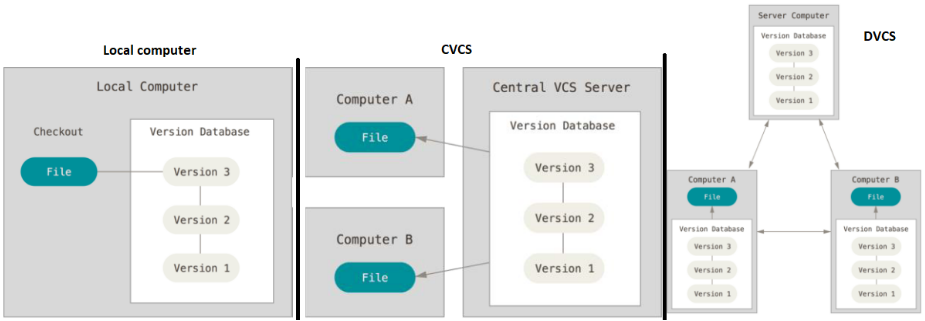
\includegraphics[width=1\textwidth]{img/version_control_comp.PNG}
	\caption{Version control on a local computer vs CVCS vs DVCS}
	\label{fig:version_control_comp}
\end{figure}

\subsection{Git}
To help with the maintenance of code during the development of software, having a full story of changes made in a data repository and also a version control over it, some applications were developed. The most used one is called GIT, which is a \ac{VCS}, created by Linus Torvalds for development of Linux kernel and ended up also being used by many other projects due to the benefits that can come from it. When the data is being saved in a git repository, nothing will be ever lost, since it is always possible to rewind to the previous results and check what was generated by the different versions of the data. In case of conflicts, like having the same code being changed by two different users and submitted to the same repository, GIT also make automatic notifications about this conflicts in a way to advice the user that he can overwrite some information. The projects saved on GIT are divided in two parts and combination of this two parts is what form a repository:

\begin{itemize} [noitemsep]
\item Files and directories of that files.
\item Extra GIT information about the data saved - this information is saved on a directory ".git" and is present in the root directory, which should never be modified to maintain the repository integrity.
\end{itemize}

It is possible also to divide the working area of GIT in three parts, the "working directory", "stagging area" and the ".git directory". The "stagging area" is a special area that takes care of the files that are on hold to be submitted (commit) to the repository.

\begin{figure}[H]
	\centering
    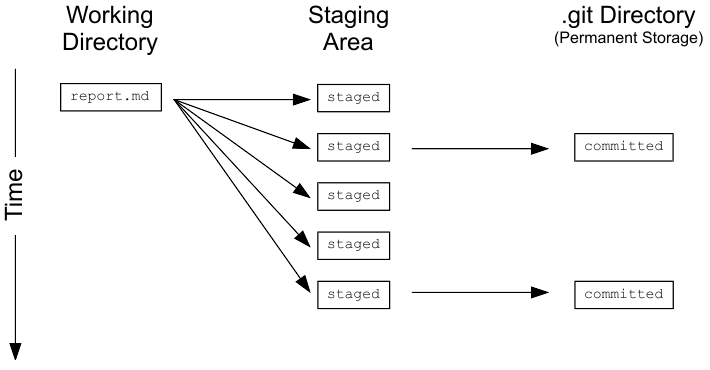
\includegraphics[width=0.8\textwidth]{img/git_areas.PNG}
	\caption{Git working areas (from datacamp.com)}
	\label{fig:git_areas}
\end{figure}

The working directory is were the current file or code is being modified. Different versions of that file can be put inside of the "stagging area", which behaves like a box were it is possible to put or take out things, but once they are submitted or "commited" to the .git directory, is not possible to make further changes on it. There are a lot of functions that can be used to manage the information inside the repository with GIT, always preceded with the "git" label. Some examples are "git status" to check the repository status, "git diff" to check the differences that have been made in the repository or between versions of files or even the "git commit" that sends the data to the repository with some extra information.

Git has a multi-level structure to save the data. After \textit{"commiting"} the data to the repository, sections and subsections are created to manage the all the data that has been sent, called "Tree" and "Blob". Each commit made to these sections, is composed by a "hash" which is a string with 40 hexadecimal characters, created randomly by a hash function. This hash gives a unique identifier to each commit sent to the repository and this enable a GIT system to share the data in a efficient way between repositories. The basis is simple: if two files are exactly the same, they will have the same hash string and vice-versa. A typical look of a hash can be "5ac632e3a1be3749e1758f195f719957a2e37e12". Since it is too big to be handled every time, when it is necessary to check or compare some commits, it can be used only the first 5 to 8 characters for that.

In the figure \ref{fig:commit_example}, is possible to see how information is being sent to repository. The commit sends the information related to the author, plus a log message (some comment made by the author) and properties of commit, like the date and hour of submission. 

\begin{figure}[H]
	\centering
    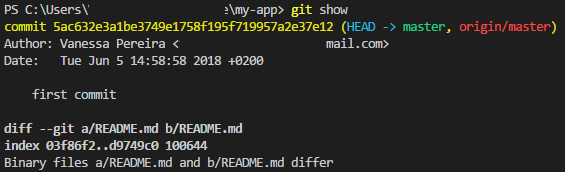
\includegraphics[width=0.7\textwidth]{img/commit_example.PNG}
	\caption{Git show commit example}
	\label{fig:commit_example}
\end{figure}

Then this information is sent to the "Tree". The tree is composed by all files names and locations commited to the repository and makes the track of these files. The "Blob" is the unique version of every file, which can contain any type of data. These blobs can be shared between trees.

\begin{figure}[H]
	\centering
    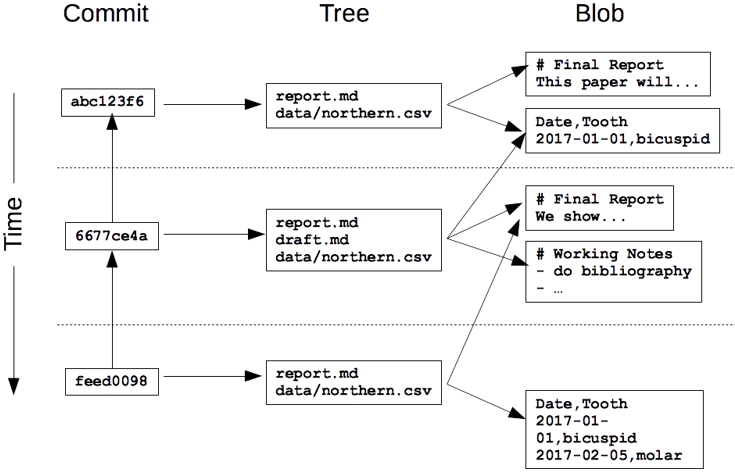
\includegraphics[width=0.9\textwidth]{img/git_commit_areas.PNG}
	\caption{Git commit composition (from datacamp.com)}
	\label{fig:git_commit_areas}
\end{figure}

Other interesting feature on GIT are the branches. In every GIT repository there is a branch called "master" where the principal workflow of data (main directory) occurs. This is also the branch on production. Then there are other branches that can be created from the master branch and will work like a sub-directory. When these "sub"-branches are created, all the data from "master" branch is replicated/copied. After the branch has been created, every change made in it, does not affect the "master", but in case of using the git command "git merge", all the changes made in this branch will get merged and then commited to the "master" branch. In case of merging branches, for example, between a master and another branch, this means that one commit made to the repository can have two parents. 

Every repository can be cloned. With this, GIT know what was the original repository and will create a remote repository pointed to the original one, usually with the name "origin" and an \ac{URL} linked to it. This is the case of having a local repository (master) and a cloned repository (origin) in online repository services like GitHub or GitLab. With git is possible to have a copy of a project in the personal computer in a offline mode, but if there are any changes that should be replicated in the distributed repositories, these changes will only be "commited" to GitHub or GitLab if there is an online access.   


\subsubsection{GitHub and GitLab}

GitHub and GitLab are web-based (or cloud-based) collaborative repositories that interacts with GIT, mostly used to save code from developers, but it can also saves another type of data. GitHub projects can be made public and shared among everyone, which are used for open source software, or this projects can also be private, if paying a plan. 
GitLab is similar to GitHub, but is more used in a enterprise environment. This is due to the authentication method - on GitHub is only possible to set permissions based on read and write access. On GitLab, it is possible to change users permissions based on their role, so controlling teams is easier. Also it provides unlimited private repositories for free. \\

Although it seems that GitLab is less popular that GitHub, it is because GitLab entered on the market few years after GitHub which already was very well positioned in this area. Both services have very solid REST API applications, that allows developers to make HTTP requests with the information that they what to get from the hosted repositories. 


\subsection{Semantic Versioning}
When a software application is being developed, it passes through many changes. During the years, the management of software suffer a lot of variations and to help dealing with this issue, a versioning guideline was made, the "semVer", which is followed by many implementers. The changes in software were hard to maintain and after some time, working along with so many new releases could be a challenging job. Within this, the "semVer" defines that each one of this changes can be divided in major, minor and patch. This divisions are labeled with a tag containing numbers separated by dots, respective to each version. For example, for an initial development release, the version should be (0.1.0). In case of the minor release, it should be incremented by 1, for example (0.2.0). When the software goes into production, the major number should increase (1.0.0). Summarizing, if it is given a version number (Major.Minor.Patch), the incrementation is made when: \citep{preston2018}
\begin{itemize} [noitemsep]
\item Major version - incompatible API changes have been made;
\item Minor version - is added functionality in a backwards-compatible manner;
\item Patch version - backwards-compatible bug fixes was made.
\end{itemize}

OpenEHR archetypes and templates are following this way to versioning the different releases. When a archetype is being revised, it takes a special number based on the “semVer” rules. Each archetype that is currently on use, has a version that follows the next schema:
\begin{itemize} [noitemsep]
\item (majorVersion.minorVersion.patchNumber) - e.g. (1.1.1).
\end{itemize}

It can also have an optional version modifier, as "alpha element" in case of being considered an unstable archetype or as "release candidate". If an archetype was never published, it will have a “majorVersion” of 0 (e.g. 0.1.1) and this is also indicated in the archetype name, preceded by ".v" (e.g. openEHR-EHR-OBSERVATION.blood\_pressure\textbf{.v0}). This procedure will be explained in detail in the chapter 3.  


\newpage

\end{document}